\documentclass{../tudscript}
\author{Jakob Krebs}
\title{Mathe VL 10}

\begin{document}
    \ssect{spezielle Ableitungen}
        \ilmath{f(x) &= x^x, x > 0 \\
                ln(f(x)) &= ln (x^x) = x \* ln x \\
                \frac{1}{f(x)} \* f'(x) &= 1 \*ln x + x \* \frac{1}{x} \\
                \implies f'(x)&= x^x \* (ln x + 1)}
        \ilmath{f(x) &= x^x = x^{e^{ln x}} \\
                \implies f'(x) &= e^{x \* ln x} (ln x + 1)}
        \ilmath{(sinh x)' &= cosh x \\
                (cosh x)' &= sinh x}
        Cosinus Hyperbolicus blau und Sinus Hyperbolicus rot:
        \ilmath{cosh x := \frac{e^x + e^{-x}}{2}}
        \begin{tikzpicture}
	        \draw[->] (-2.2,0) -- (2.2,0) node[right] {$x$};
	        \draw[->] (0,-2.2) -- (0,4.2) node[above] {$y$};
	        \draw[scale=1,domain=-2:2,smooth,variable=\x,blue] plot ({\x},{ (e^\x + e^(-\x))/(2) });
	        \draw[scale=1,domain=-1.6:2,smooth,variable=\x,red] plot ({\x},{ (e^\x - e^(-\x))/(2) });
        \end{tikzpicture}
        \\
    \ssect{Taylorreihenentwicklung für cosh x}
        \ilmath{e^x = \sum_{k = 0}^\infty \frac{x^k}{k!}}
        ist absolut konvergent für alle $x \in \bR$
        \ilmath{e^{-x} = \sum_{k = 0}^\infty \frac{(-x)^k}{k!}}
        einsetzen in cosh (x)

        \ilmath{cosh x &= \frac{e^x + e^{-1}}{2} \\
                       &= \ldots \\
                       &= \sum_{k = 0}^\infty \frac{x^{2k}}{(2k)!}}
    \ssect{spezielle Grenzwerte (Regeln von Bernoulli- L'Hospital)}
        Seien $f(x), g(x)$ reele 2- mal stetig differenzierbare Funktionen auf einem
        Intervall $(a,b)$ und $f(x_0) = f(x_0) = 0$.
        
        Gesucht: \ilmath{\lim_{x \to x_0} \frac{f(x)}{g(x)}}
        
        \ilmath{\frac{f(x_0)}{g(x_0)} &= \frac{f(x_0) + f'(x_0) (x-x_0) + \frac{1}{2} f''(x) (x-x_0)^2}{g(x_0) + g'(x_0) (x-x_0) + \frac{1}{2} g''(x_0) (x-x_0)^2} \\
                &= \frac{(x-x_0)}{x-x_0} \* \frac{f'(x_0) +  \frac{1}{2} f''(x_0) (x-x_0)}{g'(x_0) + \frac{1}{2} g''(x_0) (x-x_0)} \\
                &= \lim_{x \to x_0} \frac{f'(x_0) + \frac{1}{2} f''(x_0)}{g'(x_0) + \frac{1}{2} g''(x_0)}}


        Regel von Bernoulli-L'Hospital
        \ilmath{\boxed{\lim_{x \to x_0} \frac{f(x)}{g(x)} = \lim_{x \to x_0} \frac{f'(x)}{g'(x)}, \text{ falls GW ex.}}}

        \sssect{Beispiele}
        \ilmath{\lim_{x \to 0} \frac{sin x}{x} = \lim_{x \to 0} \frac{cos x}{1} = cos 0 = 1}
        
        \sssect{Bemerkung}
        	Diese regeln sind durch geeignetes umformen auch bei folgenden Typen anwendbar: $0 \* \infty$, $0^0$, $1^0$, $1^\infty$
        	
        \sssect{Beispiele}
        \ilmath{\lim_{x \to 0^+} x ln (x) \overset{0 \* -\infty}{=} = \frac{ln x}{\frac{1}{x}} = \lim_{x \to 0^+} = \frac{(ln x)'}{(\frac{1}{x})'} = \lim \frac{\frac{1}{x}}{\frac{-1}{x^2}} = \lim (-x) = 0} 

        \ilmath{\lim_{x \to 0} x^x  \overset{0^0}{=}  \lim e^{ln (x^x)} = \lim_{x \to 0} e^{ln(x^x)} = e^{\lim_{x \to 0} x ln x} = e^0 = 1}


        %%TODO hier bitte nach Fehlern suchen
        \ilmath{\lim_{x \to 0} x^\frac{1}{ln x} \overset{0^0}{=} \lim_{x \to 0} e^{ln (x^{\frac{1}{ln x}})} = \lim e^{\frac{1}{ln x} ln x} = \lim e^1 = e}

        \ilmath{\lim_{x \to \infty} (1+ \frac{1}{x})^x \overset{1^\infty}{=} \lim_{x \to \infty} e^{ln (1+ \frac{1}{x})^x} = \lim_{x \to \infty} e^{x \* ln (1+ \frac{1}{x})} = e^{\lim_{x \to \infty} x ln (1+ \frac{1}{x})} = e^1 = e}


        \ilmath{\lim_{x \to \infty} x ln (1 + \frac{1}{x}) = \lim_{x \to \infty} \frac{ln (1 + \frac{1}{x})}{\frac{1}{x}} \overset{\frac{0}{0}}{=} = \lim_{x \to \infty} \frac{1}{1+\frac{1}{x}} = 1}

    \sect{Integralrechnung}
        \ssect{Riemann-Integrale}
            $f(x) \geq 0$ auf $(a, b)$

            
            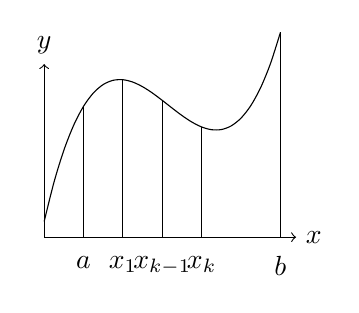
\begin{tikzpicture}
	            \draw[->] (0,0) -- (3.2,0) node[right] {$x$};
	            \draw[->] (0,0) -- (0,2.2) node[above] {$y$};
	            \draw[scale=1,domain=0:3,smooth,variable=\x,black] plot ({\x},{ 0.7*(\x-1)^3 - 1.2*(\x-1)^2 - 0.1*(\x-1) + 2 });
	            \node[label=below:$a$] at (0.5, 0) (a) {};
	            \node[label=below:$x_1$] at (1, 0) (x1) {};
	            \node[label=below:$x_{k-1}$] at (1.5, 0) (xk1) {};
	            \node[label=below:$x_k$] at (2, 0) (xk) {};
	            \node[label=below:$b$] at (3, 0) (b) {};
	            \draw[-] (0.5, 1.663) -- (0.5, 0);
	            \draw[-] (1, 2) -- (1, 0);
	            \draw[-] (1.5, 1.73) -- (1.5, 0);
	            \draw[-] (2, 1.4) -- (2, 0);
	            \draw[-] (3, 2.6) -- (3, 0);
            \end{tikzpicture}
            typisch via ober unter Summe..
            \ilmath{\lim_{||P|| \rightarrow 0} \underline{s_p} = \lim_{||P|| \rightarrow 0} \overline{s_p} \int^{b}_a f(x) dx}
        
        \ssect{Beispiel, Riemannintegral nicht anwendbar}
            \ilmath{D(x) = \begin{cases} 1, rational \\
                                         0, irrational \end{cases} auf [0, 1]}
                                     
            Riemann-Integral
           
            Da in jedem reelen Intervall liegen rationale und irrationale Zahlen.
            untersumme = 0, obersumme = 1

            Das Riemann Integral der Funktion D(x) ex. nicht. 
    		\\
        	
        	\begin{tikzpicture}
	        	\draw[->] (0,0) -- (3.2,0) node[right] {$x$};
	        	\draw[->] (0,0) -- (0,2.2) node[above] {$y$};
	        	\draw[] (0, 2) -- (0.5, 2) -- (0.5, 0);
	        	\draw[] (0.5, 1.5) -- (1, 1.5) -- (1, 0);
	        	\draw[] (1, 0.5) -- (1.5, 0.5) -- (1.5, 0);
	        	\draw[] (1.5, 0) -- (1.5, 1) -- (2, 1) -- (2, 0);
	        	\draw[] (2, 0) -- (2, 2) -- (2.5, 2) -- (2.5, 0);
	        	\draw[] (2.5, 1) -- (3, 1) -- (3, 0);
        	\end{tikzpicture}
            $\varphi$ ist eine Treppenfunktion

            \ilmath{\int_a^b \varphi(x) = \sum c_k \*(x_k - x_{k-1})}
            \begin{center}
            \enquote{Und der Rest ist jetzt eigentlich ganz einfach, wenn man die Details weg lässt.}
    \end{center}
            \ilmath{\lim_{k \to \infty} \int_a^b \varphi_k (x) = \int_a^b f(x) dx}
            ist das Lebesgue Integral.                    
             
\end{document}
